\documentclass[main.tex]{subfiles}

\begin{document}

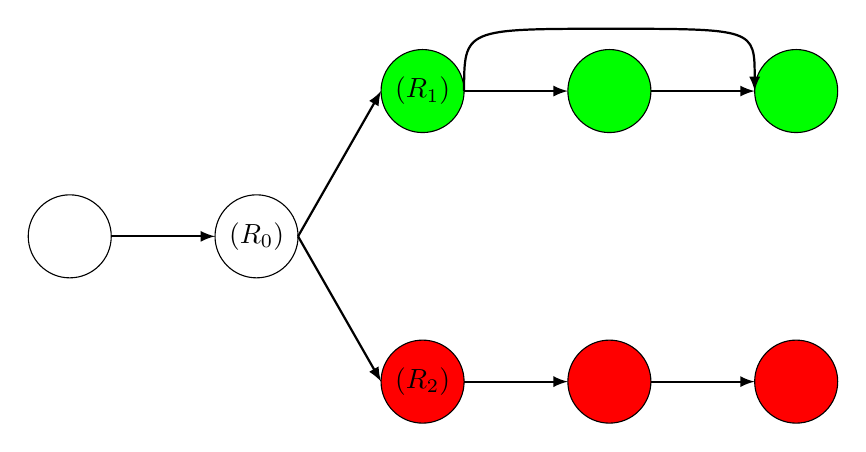
\begin{tikzpicture}[x=0.75pt,y=0.75pt,yscale=-1,xscale=1]

% black path
\draw [fill={rgb, 255: red, 0; green, 0; blue, 0}, fill opacity=0] (10, 100) circle (20);

\draw [fill={rgb, 255:red, 0; green, 0; blue, 0 }, fill opacity=1, ->, >=latex,thick,black] (30, 100) -- (80, 100);

\draw [fill={rgb, 255: red, 0; green, 0; blue, 0}, fill opacity=0 ] (100, 100) circle (20);
\draw (100, 100) node  [align=left] {($R_0$)};

% Green path
\draw [fill={rgb, 255: red, 0; green, 255; blue, 0}, fill opacity=1] (180, 30) circle (20);
\draw (180, 30) node  [align=left] {($R_1$)};

\draw [->, >=latex,thick,black] (200, 30) -- (250, 30);

\draw [fill={rgb, 255: red, 0; green, 255; blue, 0}, fill opacity=1] (270, 30) circle (20);

\draw [->, >=latex,thick,black] (290, 30) -- (340, 30);

\draw [fill={rgb, 255: red, 0; green, 255; blue, 0}, fill opacity=1] (360, 30) circle (20);

\draw [->, >=latex,thick,black] (200, 30) .. controls (200, 0) and (200, 0) .. (270, 0) .. controls (340, 0) and (340, 0) .. (340,30);


% Red path
\draw [fill={rgb, 255: red, 255; green, 0; blue, 0}, fill opacity=1] (180, 170) circle (20);
\draw (180, 170) node  [align=left] {($R_2$)};

\draw [->, >=latex,thick,black] (200, 170) -- (250, 170);

\draw [fill={rgb, 255: red, 255; green, 0; blue, 0}, fill opacity=1] (270, 170) circle (20);

\draw [->, >=latex,thick,black] (290, 170) -- (340, 170);

\draw [fill={rgb, 255: red, 255; green, 0; blue, 0}, fill opacity=1] (360, 170) circle (20);

% Link between path
\draw [->, >=latex,thick,black] (120, 100) -- (160, 30);

% Link between path
\draw [->, >=latex,thick,black] (120, 100) -- (160, 170);

\end{tikzpicture}

\end{document}

